\documentclass[a4paper,11pt]{article}
\usepackage[latin1]{inputenc}
\usepackage[T1]{fontenc}
\usepackage{amsmath}
\usepackage{a4wide}
\usepackage{booktabs}
\usepackage{graphicx}

\title{Genomics and Bioinformatics}
\date{October 29, 2013}
\author{Examination - Week 7}
\begin{document}
\maketitle

\section*{Question 1 - Genome Assembly}

Consider the following reads:
ATGATGC, TGCATGA, ATGCCAT, CCATGCA

\begin{enumerate}
\item Construct the overlap graph based on the above reads, using an
  overlap size of $4$ bases.
  Draw a path that goes
  through every \emph{vertex} (Hamiltonian path), and write the
  corresponding contig. 
\item Make a list $S_4$ of all unique $4$-mers (10 elements) and the
  list $S_5$ of all (non-unique) 5-mers (12 elements). 
\item Construct the De Bruijn graph with $S_4$ as vertex set and
  $S_5$ as edge set.
\item Is this graph Eulerian?
\item Find two Eulerian paths, write down the corresponding contigs,
  and indicate which of them is incompatible with the full reads.
\end{enumerate}


\section*{Question 2 - Sequence Alignment}

\subsection*{Linear gap penalty}
Using the following scoring: a match is worth 2 points, a mismatch is penalized -1,
and a gap is penalized -2 points, find 3 optimal alignments of the sequences\\
\texttt{AACTTTG}, \texttt{ACCTG}\\
by the Needleman-Wunsch algorithm. What is their score ? 


\subsection*{Affine gap penalty}

Calculate the scores of the previous alignments using a gap opening penalty of -2 points. 
Are the previous alignments still equivalent?

\section*{Question 3 - Hidden Markov Model}

\begin{figure}[h]
\center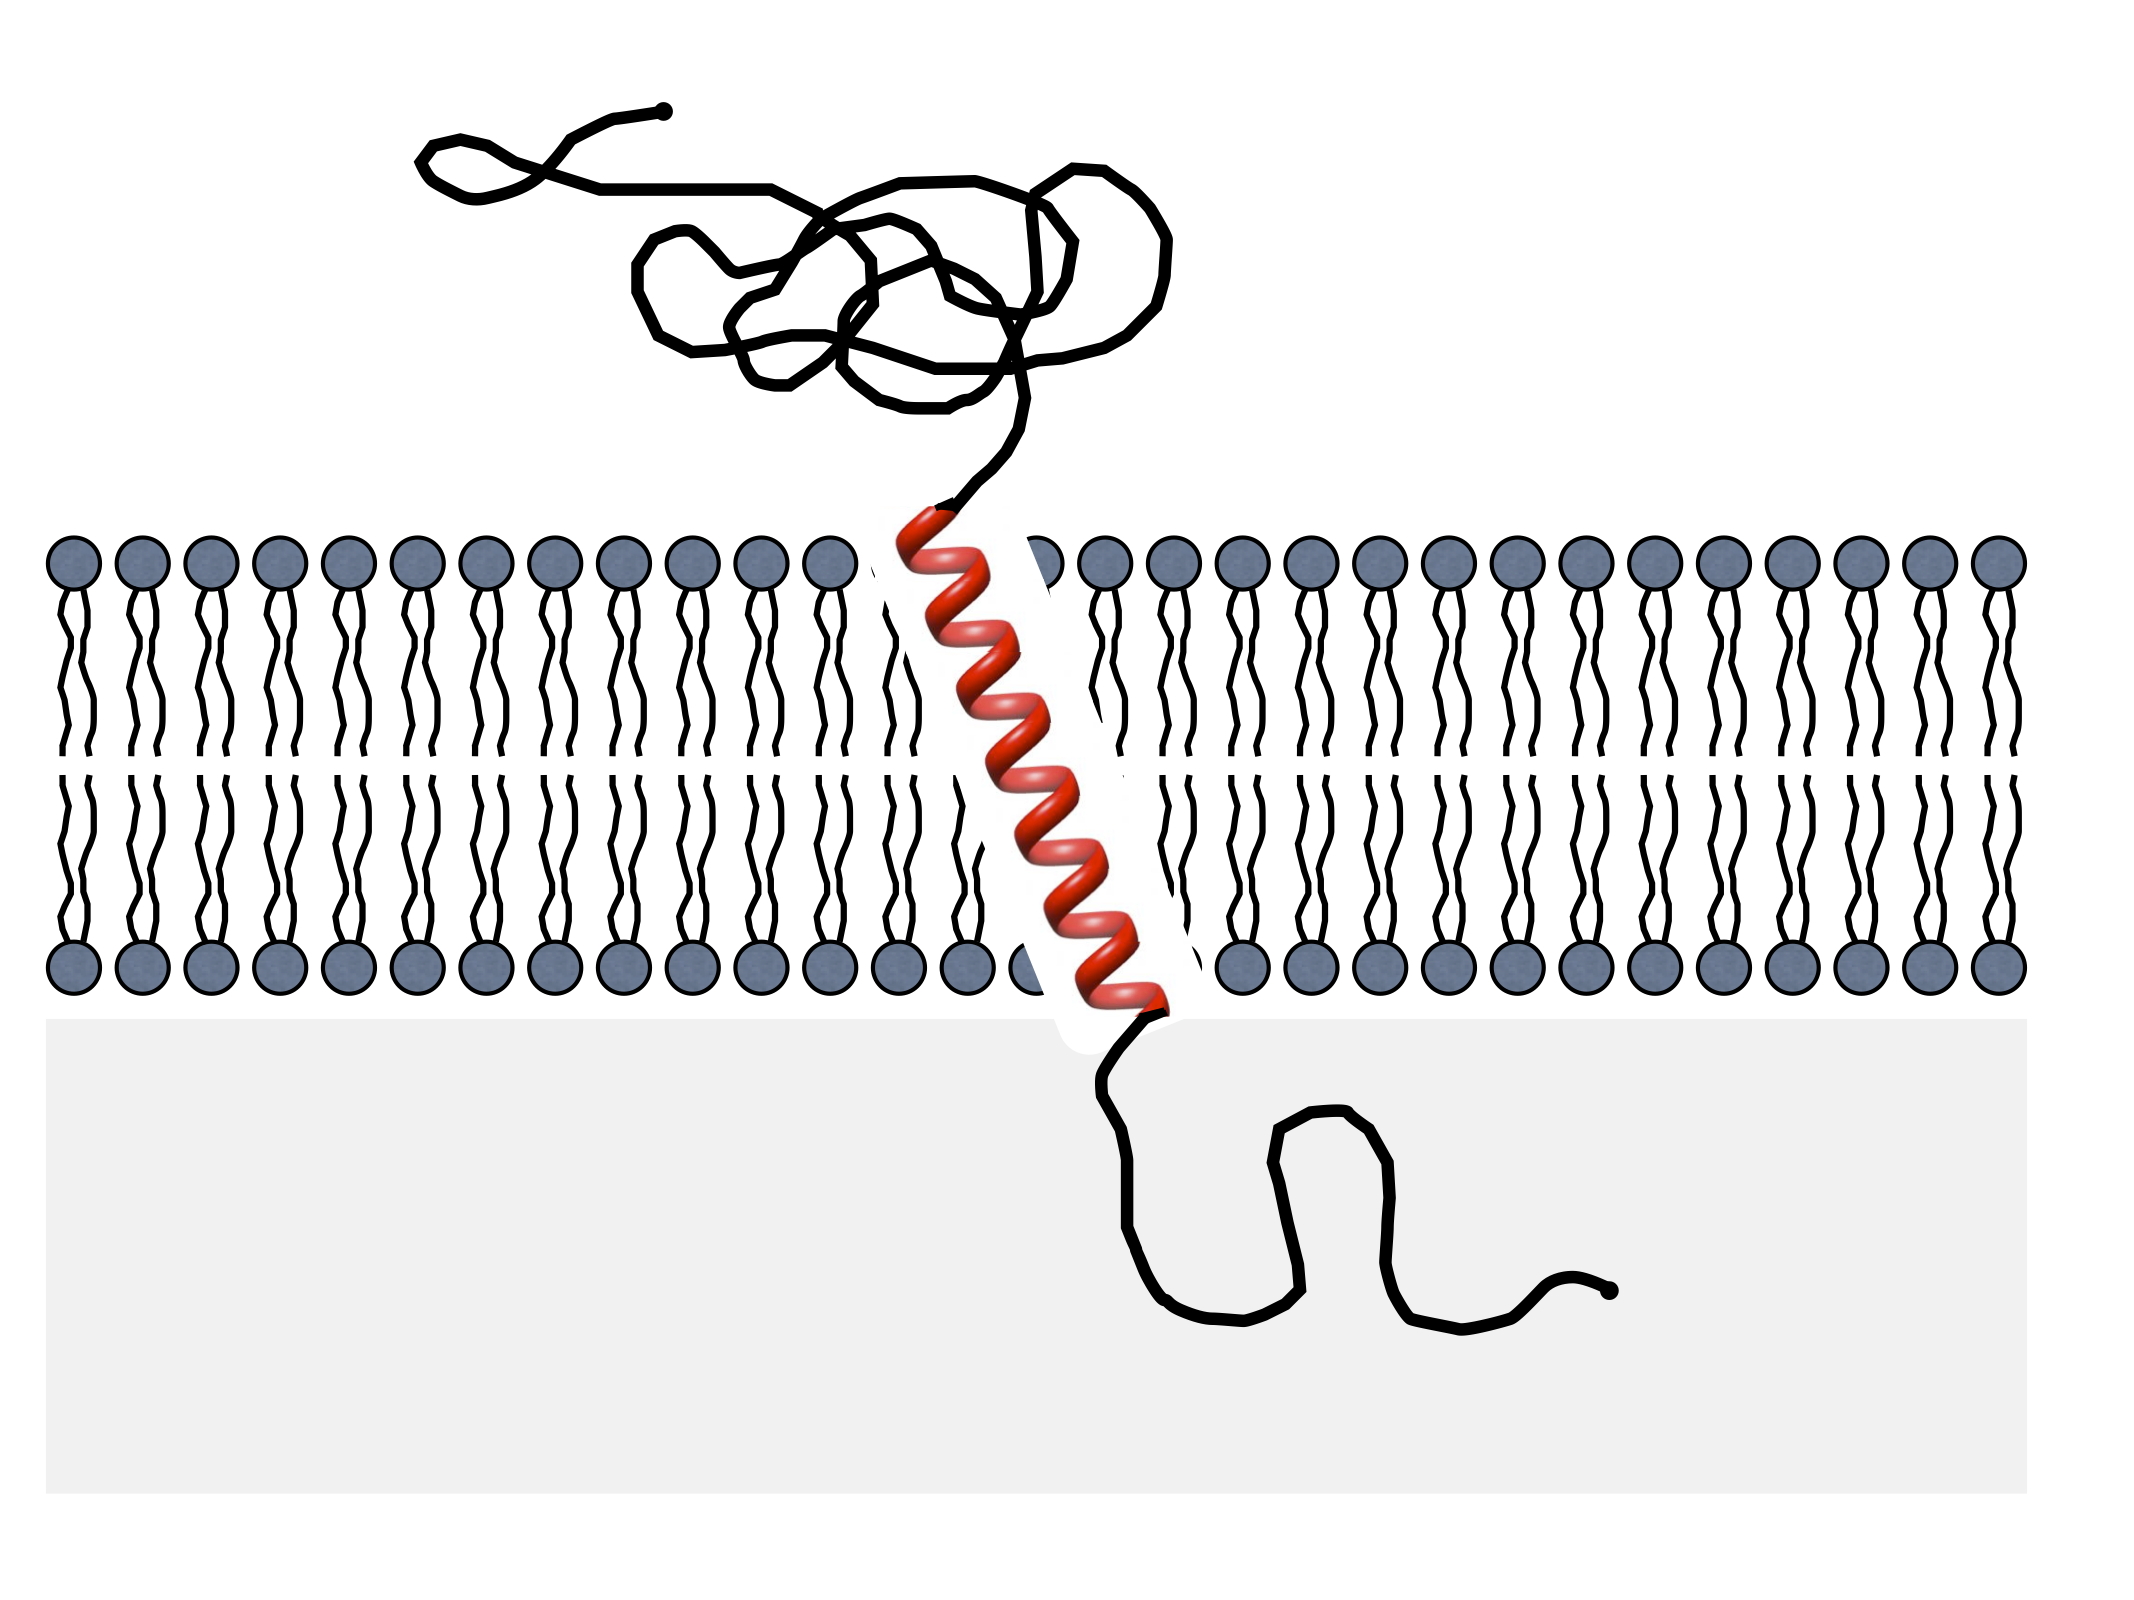
\includegraphics[scale=.2]{transmembrane.png}
\end{figure}

A transmembrane protein is a protein with one or more domains going from one side of the 
plasmic membrane through to the other side. As a consequence, it contains
extracellular, intracellular and transmembrane domains. 
Very often the transmembrane domains are structures 
known as ``alpha-helices''. 
We want to find them using a Hidden Markov Model.

The propensity of different amino-acids to be part of an alpha-helix
is well-known and scored in the table below.
For this exercise we assume that 
\begin{itemize}
\item Transmembrane domains are alpha-helices of 20 amino-acids on average. 
\item Amino-acids are equally distributed in the other domains.
\item Intracellular domains are 200 amino-acids long on average 
and extracellular domains, 400 amino-acids.
\end{itemize}

\begin{table}[h]
 \caption{Frequency of amino-acids within helical domains:}
  \begin{center}
    \begin{tabular}{ cccccccccc c }
      A & R & N & D & C & E & Q & G & H & I \\
      \bf{8\%} & 7\% & 4\% & 4\% & 4\% & 6\% & 6\% & 3\% & 5\% & 6\% \\
    \\
      L & K & M & F & P & S & T & W & Y & V \\
      7\% & 6\% & 7\% & 5\% & \bf{0.3\%} & 5\% & 4\% & 5\% & 5\% & 5\% \\
    \end{tabular}
  \end{center}
\end{table}


\begin{enumerate}
\item Propose a simple Hidden Markov Model to predict transmembrane domains 
from a given amino-acids sequence (draw a diagram).
\item What are the emission probabilities?
\item Based on the length of the respective domains, give an estimate
  of the transition probabilities. Write the transition matrix.
\item Here is the sequence of a dummy transmembrane protein. How would
  you calculate the probability of observing this sequence, given the
  model? (Do not calculate it).
$$\mbox{NGAKTTL}$$

\item On the same protein, we underlined the transmembrane domain. 
What is the probability of observing this sequence? 
$$\mbox{NG\underline{AK}TTL}$$

\item \textit{Bonus:} how would you adapt the model (only the diagram)
  if moreover you know that an alpha-helix is defined as hydrogen
  bonds linking groups of 4 amino-acids?
\end{enumerate}

\section*{Question 4 - Homology}


Toll-like receptors (TLRs) are a class of proteins involved in the innate immune system. 
They all share similarity to the \textit{Drosophila} protein Toll and
are found in vertebrate and non-vertebrate species.  
Some of their motifs can be found in plants and bacteria, suggesting
that they are components of an ancient immune system. 

The table below provides BLAST scores of pairwise
alignments for six TLR family proteins (from 3 different species) and
the \textit{Drosophila} Toll protein,  

\begin{enumerate}
\item {\bf TLR4\_BT} from {\it Bos taurus}, i.e. bovine,
\item {\bf TOLL\_DM} from {\it Drosophila melanogaster}, i.e. fruit fly,
\item {\bf TLR3\_HS} and {\bf TLR4\_HS} from {\it Homo sapiens}, i.e. human,
\item {\bf TLR3\_MM} and  {\bf TLR4\_MM} from {\it Mus musculus}, i.e. mouse.
\end{enumerate}

\begin{center}
	\begin{tabular} {| l || l | l | l | l | l | l |}
	\hline
 	                    & TLR4\_BT&TOLL\_DM & TLR3\_HS& TLR4\_HS&  TLR3\_MM& TLR4\_MM\\ \hline\hline
	TLR4\_BT        & -            & 460             &  177         & 1263       &205           & 1061 \\	\hline
	TOLL\_DM      & 412       & -                  &  188        & 358       & 150           & 404 \\	\hline
	TLR3\_HS       & 169      & 255              & -             & 160       &1406           & 117 \\	\hline
	TLR4\_HS       &1238      & 375              & 166        & -            & 206           & 1087 \\	\hline
	TLR3\_MM    & 169      & 120              & 1422      & 235       & -                & 186 \\ 	\hline
	TLR4\_MM    & 1041      & 413              & 133        & 1074       & 102           & - \\
	\hline
	\end{tabular}
\end{center}
\vspace{0.05 cm}

\begin{enumerate}
\item Based on the table above, draw the gene tree for the six proteins.
  Indicate speciation and duplication events on the graph.
\item Using this tree, give examples of:
  \begin{itemize} 
  \item one orthologous pair, 
  \item one paralogous pair in the same species, and 
  \item one paralogous pair in different species.
  \end{itemize}
\end{enumerate}

\end{document}
